\begin{frame}[t]{\secname}{\subsecname}
  
\begin{itemize}
  \item Hex: $dx=\SI{0.4}{\milli\meter}$, $\delta=\SI{1.2}{\milli\meter}$
\end{itemize}

\begin{columns}[t]
  \begin{column}{0.375\textwidth}
    \only<1->{
      \begin{block}{Force-Displacement plot}
        \centering
        % Size
        \setlength{\figheight}{0.75\textheight}
        % Data
        \pgfplotstableread[col sep=comma]{\materialpath/Data/Numerics/Hex_0-4_1-2_Stoch.csv}{\loadedtable}
        % Chart
        \tikzexternalenable
        \tikzsetnextfilename{Hex_0-4_1-2_Stoch}
        \begin{tikzpicture}
          \begin{axis}[
            %height=\figheight+\baselineskip,
            height=\figheight,
            width=\linewidth,
            axis lines=middle,
            cycle list name=color list,%linestyles*,
            %cycle list shift=1,
            xmin=0,
            ymin=0,
            title=\empty,
            %xlabel={Displacement $[\si{\milli\meter}]$},
            %ylabel={Force $[\si{\newton}]$},
            xlabel={$u$ $[\si{\milli\meter}]$},
            ylabel={$F$ $[\si{\newton}]$},
            %x label style={at={(axis description cs:0.5,-0.075)},anchor=north},
            %y label style={at={(axis description cs:-0.105,0.5)},rotate=90,anchor=south},
            label style={font=\figurefontsize},
            %legend pos=south west,
            legend cell align={left},
            legend style={
              font=\figurefontsize,
              at={(0.025,0.85)},
              anchor=north west,
            },
            ticklabel style={font=\figurefontsize},
          ]%   each nth point={2}
            \addplot+ [thick] table[x=DxNo, y=FxNo] {\loadedtable};
            \addlegendentry{No stochastics}
            \addplot+ [] table[x=DxSto1, y=FxSto1] {\loadedtable};
            \addlegendentry{Stochastic 1}
            \addplot+ [] table[x=DxSto2, y=FxSto2] {\loadedtable};
            \addlegendentry{Stochastic 2}
            \addplot+ [] table[x=DxSto3, y=FxSto3] {\loadedtable};
            \addlegendentry{Stochastic 3}
          \end{axis}
        \end{tikzpicture}
        \tikzexternaldisable
      \end{block}
    }
  \end{column}
  \begin{column}{0.625\textwidth}
    \only<2->{
      \begin{block}{Failure patterns}
        \setlength{\figheight}{0.625\textheight}
        \figurefontsize
        \begin{tabular}{@{}c@{}c@{}c@{}c@{}c@{}}
        \begin{minipage}[t][\figheight]{0.1925\linewidth}
          \centering
          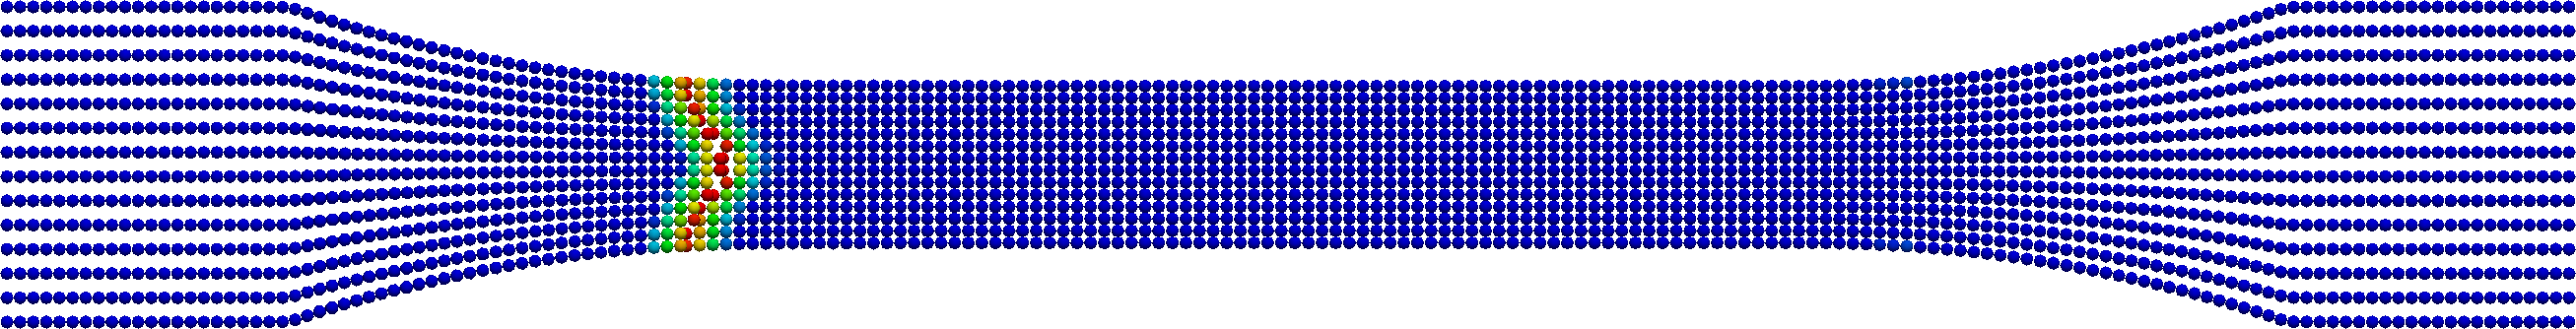
\includegraphics[angle=90,width=\linewidth,height=\figheight,keepaspectratio]{PD_Hex_Damage_0-4_1-2_3630_-z_ct}
        \end{minipage}
        &
        \begin{minipage}[t][\figheight]{0.1925\linewidth}
          \centering
          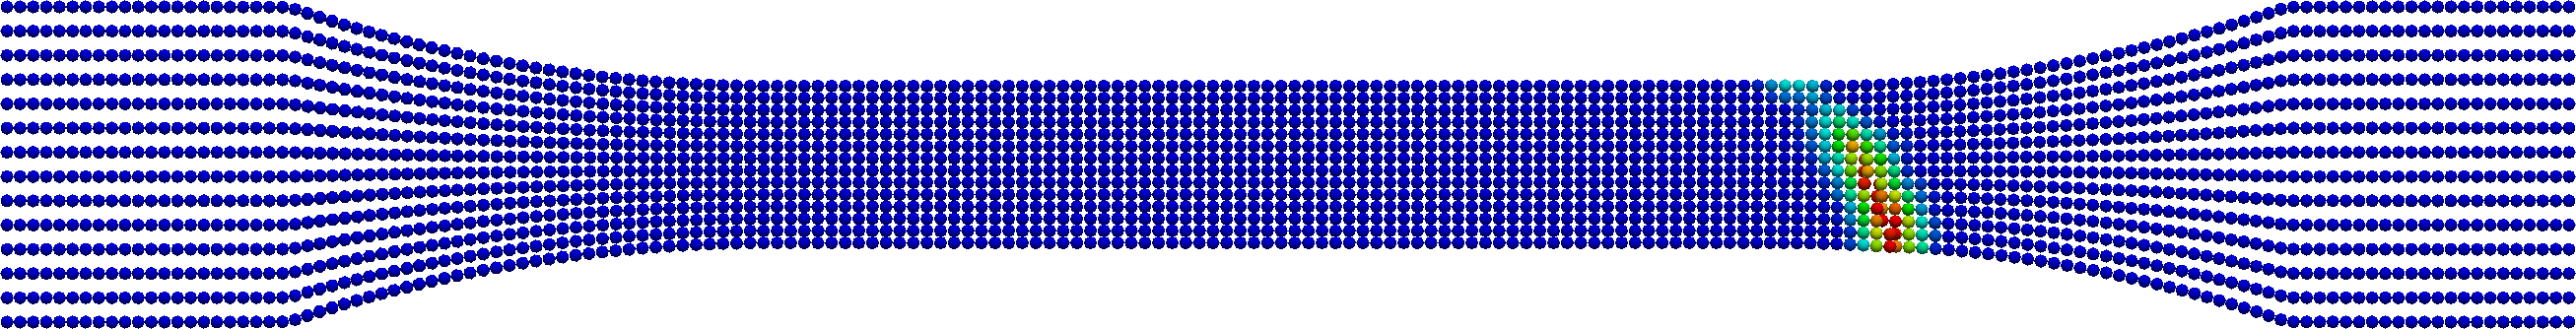
\includegraphics[angle=90,width=\linewidth,height=\figheight,keepaspectratio]{PD_Hex_Stoch_1_Damage_0-4_1-2_3475_-z_ct}
        \end{minipage}
        &
        \begin{minipage}[t][\figheight]{0.1925\linewidth}
          \centering
          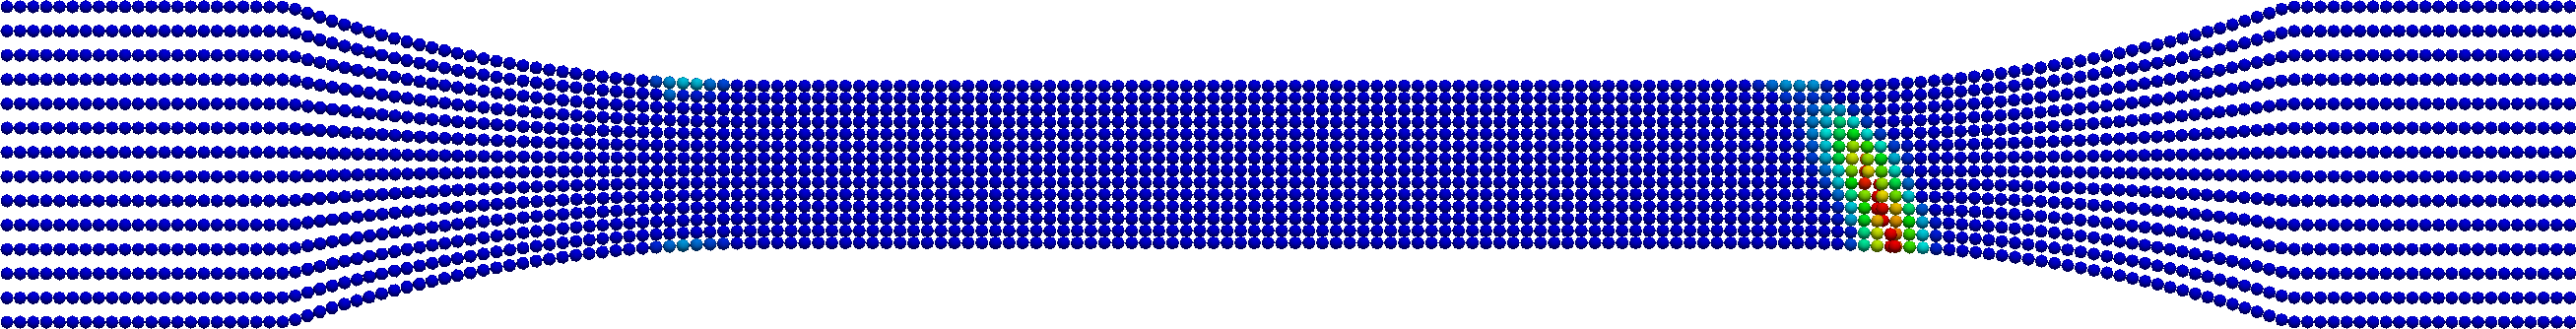
\includegraphics[angle=90,width=\linewidth,height=\figheight,keepaspectratio]{PD_Hex_Stoch_2_Damage_0-4_1-2_3540_-z_ct}
        \end{minipage}
        &
        \begin{minipage}[t][\figheight]{0.1925\linewidth}
          \centering
          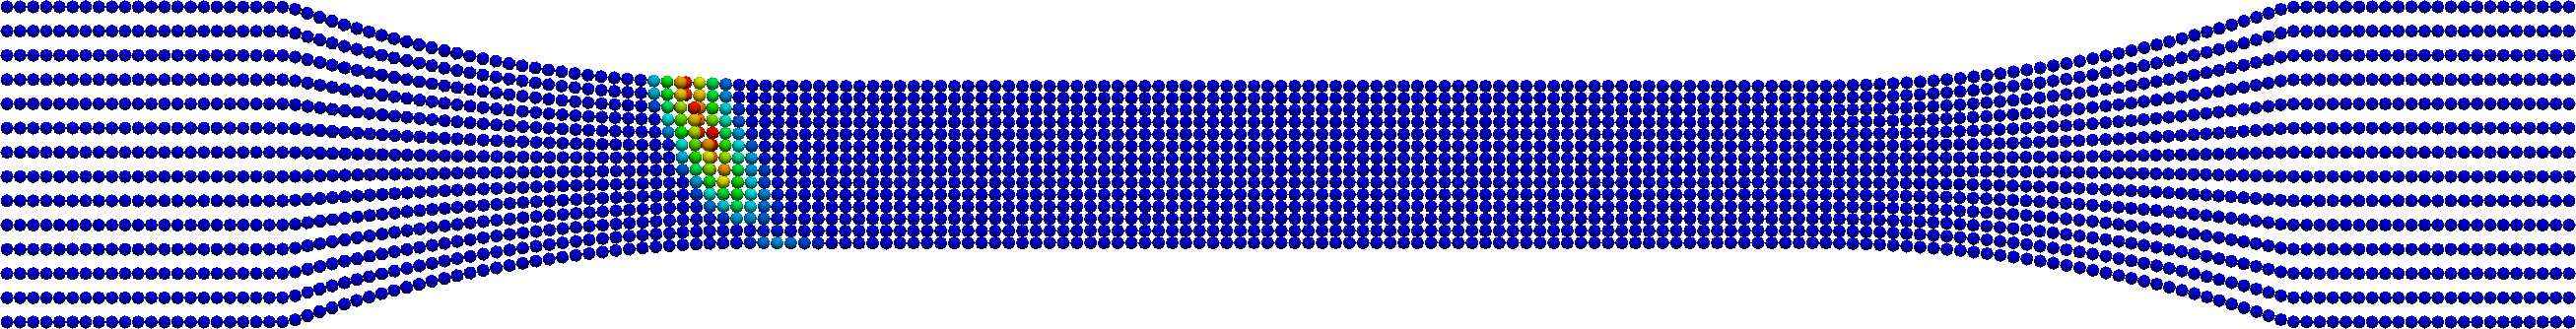
\includegraphics[angle=90,width=\linewidth,height=\figheight,keepaspectratio]{PD_Hex_Stoch_3_Damage_0-4_1-2_3292_-z_ct}
        \end{minipage}
        &
        \begin{minipage}[t][\figheight]{0.1925\linewidth}
          \centering
          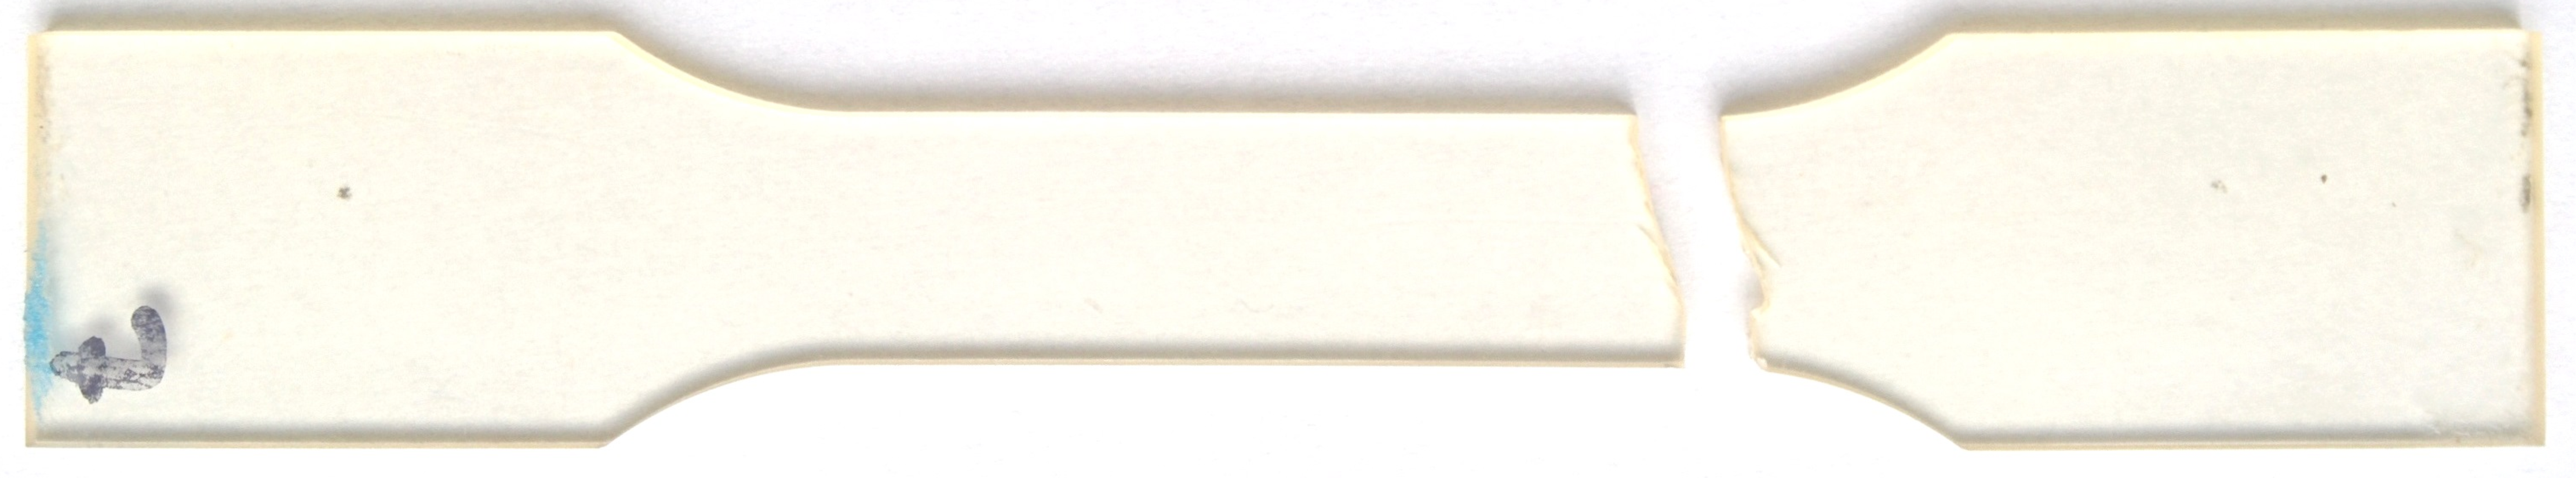
\includegraphics[angle=90,width=\linewidth,height=\figheight,keepaspectratio]{KrauseD_Damage_LY564_statisch}
        \end{minipage}\\
        No & 1 & 2 & 3 & \cite{KrauseD2016}
        \end{tabular}
      \end{block}
    }
  \end{column}
\end{columns}

\end{frame}
